% The Higgs mechanism plays a vital role in the Standard Model for explaining how gauge bosons obtain mass. The Standard Model would otherwise predict these particles to be massless. Through interactions with the Higgs field that permeates all space and whose elevated potential at zero field leads to spontaneous symmetry breaking (SSB), gauge bosons also experience symmetry breaking, causing them to acquire mass.
% See https://tikz.netlify.app/maxican-hat for a very similar image.

\documentclass{standalone}
\usepackage{pgfplots}
\pgfplotsset{compat=1.8}

\begin{document}
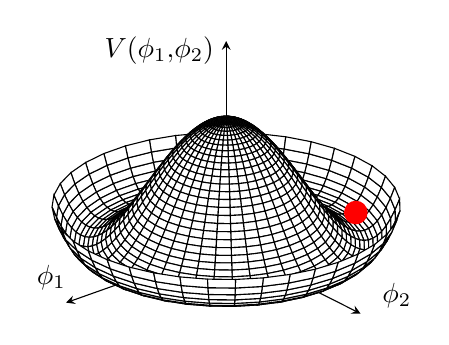
\begin{tikzpicture}
  \begin{axis}[
      axis lines=center,
      view={140}{25},
      axis equal,
      domain=0:360,
      y domain=0:1.25,
      xmax=1.5,ymax=1.5,zmin=0,zmax=1.5,
      x label style={at={(axis description cs:0.18,0.29)},anchor=north},
      y label style={at={(axis description cs:0.82,0.25)},anchor=north},
      z label style={at={(axis description cs:0.38,0.8)},anchor=north},
      xlabel = $\phi_1$,
      ylabel=$\phi_2$,
      zlabel=$V(\phi_1 \rm{,} \phi_2)$,
      ticks=none,
      clip bounding box=upper bound
    ]
	
    \addplot3 [surf,draw =black,shader = flat,opacity =1, fill =white,samples = 40, z buffer=sort,colormap/cool] ({sin(x)*y}, {cos(x)*y}, {(y^2-1)^2});
    
    %\addplot3[domain = 0:pi,red,samples = 50]({sin(deg(x))}, {cos(deg(x))}, {0.05});
     %\draw[->] (2,2,5)--(3,3,10) ;
     
  \end{axis}
  %\fill[blue] (3.47,3.5) circle [radius=0.15cm];
  \fill[red] (5.1,2.2) circle [radius=0.15cm];
  

  %\node[anchor=east] at (4.05,3.71) (text) {A};
 % \node[anchor=west] at (5.5,3.0) (description) {B};
  %\draw (description) edge[out=180,in=0,<-] (text);
  
\end{tikzpicture}
\end{document}